\documentclass[conference]{IEEEtran}
\IEEEoverridecommandlockouts
% The preceding line is only needed to identify funding in the first footnote. If that is unneeded, please comment it out.
% \usepackage{cite}
\usepackage{amsmath,amssymb,amsfonts}
\usepackage{algorithmic}
\usepackage{graphicx}
\usepackage{textcomp}
\usepackage{float}
% \usepackage{xcolor}
\usepackage[usenames,dvipsnames]{color}
\def\BibTeX{{\rm B\kern-.05em{\sc i\kern-.025em b}\kern-.08em
    T\kern-.1667em\lower.7ex\hbox{E}\kern-.125emX}}
    
\usepackage[sorting=none, style=ieee]{biblatex}
\addbibresource{bib.bib}

% \usepackage{caption}
\usepackage{subcaption}
\usepackage{placeins}

\usepackage{blindtext}
\usepackage{hyperref}
\usepackage[acronym]{glossaries}
\newacronym{ml}{ML}{Machine Leaning}
\newacronym{dl}{DL}{Deep Leaning}
\newacronym{bmi}{BMI}{Body Mass Index}
\newacronym{knn}{KNN}{K-nearest neighbors}
\newacronym{svc}{SVC}{Support Vector Classifier}
\newacronym{dnn}{DNN}{Deep Neural Network}
\newacronym{cnn}{CNN}{Convolution Neural Network}
\newacronym{dcnn}{DCNN}{Deep Convolution Neural Network}
\newacronym{acgan}{ACGAN}{Auxiliary Classifier Generative Adversarial Network}
\newacronym{ct}{CT}{Computed Tomography}
\newacronym{mri}{MRI}{Magnetic Resonance Imaging}
\newacronym{xray}{X-ray}{Radiography}

\newcommand{\TODO}[1]{\colorbox{Red}{TODO #1}}

\begin{document}

\title{Pneumonia detection with chest X-ray images using Machine Learning models}

\author{\IEEEauthorblockN{João Carvalho (106310)}
\IEEEauthorblockA{\textit{DETI} \\
\textit{University of Aveiro}\\
Aveiro, Portugal \\
jpmffc@ua.pt}
\and
\IEEEauthorblockN{João Santos (76912)}
\IEEEauthorblockA{\textit{DETI} \\
\textit{University of Aveiro}\\
Aveiro, Portugal \\
santos.martins.joao@ua.pt}
}

\maketitle

\begin{abstract}
Machine learning models applied in the medical fields as been study for many year. Yet, with the recent COVID-19 pandemic requiring novel, faster and cheaper diagnosis methods, artificial intelligence gained new strengths in this field. In this work, a study will be carried out to access the efficiency and applicability of machine learning in the early diagnosis of pneumonia and COVID-19. Multiple methods will be implemented and compared against each other, namely by using the transfer learning technique. Although this technique seamed to indicate a potential benefit over simpler convolution neural network models, a clear advantage was not proved.
\end{abstract}

\begin{IEEEkeywords}
Pneumonia, Machine Learning, Deep Learning, COVID-19, EfficientNet, transfer learning
\end{IEEEkeywords}

\section{Introduction}

Acute pulmonary infections like pneumonia can be brought on by bacteria, viruses, or fungi. When pneumonia infects the lungs, it inflames the air sacs and results in pleural effusion, which is when the lung becomes flooded with fluid.
% Pneumonia is an acute pulmonary infection that can be caused by bacteria, viruses, or fungi and infects the lungs, causing inflammation of the air sacs and pleural effusion, a condition in which the lung is filled with fluid. 
%
Pneumonia accounts for 14\% of deaths in children under the age of five years \cite{who_pneumonia}. 

The majority of cases of pneumonia occur in underdeveloped and developing nations, where there is a shortage of medical resources, excessive population, pollution, and unhygienic environmental conditions.
% Pneumonia is most common in underdeveloped and developing countries, where overpopulation, pollution, and unhygienic environmental conditions exacerbate the situation, and medical resources are scanty. 
%
Therefore, preventing the disease from becoming fatal can be greatly assisted by early diagnosis and management. For diagnosis, radiological imaging of the lungs using \gls{ct}, \gls{mri}, or \gls{xray} is frequently used. An affordable, non-invasive way to examine the lungs is via \gls{xray} images.
% Therefore, early diagnosis and management can play a pivotal role in preventing the disease from becoming fatal. Radiological examination of the lungs using \gls{ct}, \gls{mri}, or \gls{xray} is frequently used for diagnosis. \gls{xray} imaging constitutes a non-invasive and relatively inexpensive examination of the lungs. 
%
However, subjective variability might occur during chest scans \cite{neuman2012variability, williams2013variability}. As a result, the detection of pneumonia must be automated.
% However, chest X-ray examinations for pneumonia detection are prone to subjective variability \cite{neuman2012variability, williams2013variability}.  Thus, an automated system for the detection of pneumonia is required.

Deep learning is a powerful tool for artificial intelligence that is essential to the resolution of many challenging computer vision issues. Many different picture categorization issues are solved using deep learning models, particularly \glspl{cnn}.
% Deep learning is an important artificial intelligence tool, which plays a crucial role in solving many complex computer vision problems. Deep learning models, specifically \glspl{cnn}, are used extensively for various image classification problems. 

However, these models only operate at their best when they are given a lot of data. It is challenging to obtain such a large amount of labeled data for biomedical image classification problems because doing so necessitates paying expensive and time-consuming medical professionals to classify each image. A solution to get around this problem is transfer learning.
% However, such models perform optimally only when they are provided with a large amount of data. For biomedical image classification problems, such a vast amount of labeled data is difficult to acquire because it requires that expert doctors classify each image, which is an expensive and time-consuming task. Transfer learning is a work-around to surmount this obstacle.

Transfer learning is the approach of using the pertinent components of a machine learning model that has already been trained to solve a different but related problem. 

\section{State of the Art}

\gls{ml} models applied to \gls{xray} images for disease detection is not a new field of study \cite{albahli2021ai, albahli2021identification}. Yet, regarding the pandemic of the past couple of years, this field gained some focus once again in the effort to detect the damages causes by the COVID-19 disease.

\cite{chowdhury2020can} applied data augmentation to a dataset that included 423 COVID-19, 1485 viral pneumonia and 1579 healthy \gls{xray} images. With various \gls{cnn} architectures, including MobileNetv2, SqueezeNet, ResNet18, ResNet101, DenseNet201, CheXNet, Inceptionv3, and VGG19 with ImageNet trained weights. The authors also used transfer learning techniques. When only considering the COVID-19 and healthy images, this methodology provided an accuracy of 0.997, a precision of 0.997 and an F1-score of 0.997. On the other hand, if the viral pneumonia images were also considered, the results drop down to an accuracy of 0.979, a precision of 0.975 and an F1-Score of 0.979.

\cite{waheed2020covidgan} carried out the classification of COVID-19 \gls{xray} images using the \gls{acgan} technique. The authors resized the input images to a size of $112 \times 112$ and fine-tuned the fully connected layer weights. The author added data augmentation to a dataset that already contained 721 images of the healthy and 403 images of COVID-19 during the preprocessing stage. This approach reached an accuracy of 0.960. Although the results of this study are encouraging, the significant reduction of the size of the images may have result on the loss of key information.

\cite{brunese2020explainable} applied a technique that uses VGG16 \gls{cnn} architecture to highlight specific chest radiography regions to identify pneumonia. 250 COVID-19, 3520 healthy and 2753 pneumonia images were classified in their study, achieving a F1-Score of 0.940 and an accuracy of 0.960. Despite the positive outcome, the authors choose not to investigate additional options, such as image preprocessing.

Three \gls{dcnn} architectures were used in the suggested method by \cite{narin2021automatic}. The authors used a dataset with 50 healthy and 50 COVID-19 patients \gls{xray} images, all of which were resized to $224 \times 224$. The authors employed transfer learning models to get around the issue of the small dataset. The developed DCNN was based on pre-trained models that could recognize COVID-19 from standard \gls{xray} images (ResNet50, Inception V3, and Inceptio ResNet V2). The obtained results demonstrated that the pre-trained ResNet50 model provided an accuracy of around 0.980.

\cite{farooq2020covid} proposed a \gls{cnn} framework to distinguish COVID-19 cases from other Pneumonia (bacteria and virus) and healthy cases, using the COVDIX dataset \cite{wang2020covid} (which included 5941 chest \gls{xray} images from 2839 patients). Using a cyclical learning rate, the accuracy achieved was of 0.962.

Also using chest \gls{xray} images, \cite{zhang2020covid} demonstrated a \gls{dl} model that could distinguish COVID-19 from healthy individuals. Three elements formed the basis of the model: The first is a residual \gls{cnn} with 18 layers called the backbone network. The principle is to take the chest \gls{xray} image and extract the high-level features from it. The second one is powered by the extracted features and is responsible for generating a classification score while the third and last one detects anomalies and outputs an anomaly score. With both scores, the classification is done using a threshold value.

\section{Data Description}

The dataset used in the current project was available in Kaggle \cite{kolas_2022}. The referred dataset is composed by \gls{xray} images of patients that have been diagnosed with COVID-19 (1281 images), viral-pneumonia (1656 images), bacterial-pneumonia (3001 images) and that are healthy (3270 images). These images originate from multiple sources (without duplicates) and because so, have different sizes, brightnesses and ratios, as shows on Fig. \ref{fig:dataset_examples}.

\begin{figure}[htp]
    \centering
    \begin{subfigure}[b]{0.35\textwidth}
         \centering
         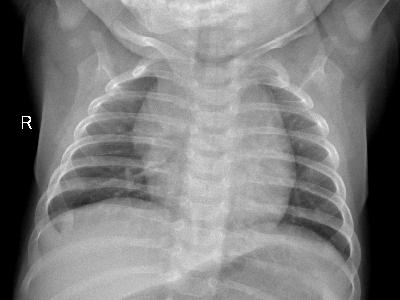
\includegraphics[width=\textwidth]{imgs/Normal (1).jpg}
         \caption{}
         \label{fig:example_normal}
     \end{subfigure}
     \hfill
     \begin{subfigure}[b]{0.35\textwidth}
         \centering
         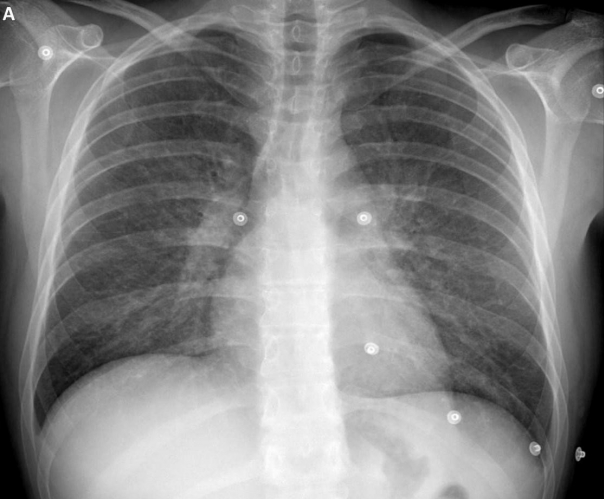
\includegraphics[width=\textwidth]{imgs/COVID-19 (1).jpg}
         \caption{}
         \label{fig:example_covid19}
     \end{subfigure}
     \hfill
     \begin{subfigure}[b]{0.35\textwidth}
         \centering
         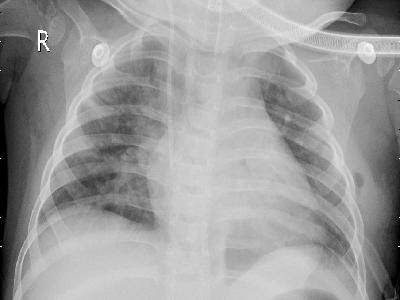
\includegraphics[width=\textwidth]{imgs/Pneumonia-Bacterial (1).jpg}
         \caption{}
         \label{fig:example_pneumonia_bact}
     \end{subfigure}
     \hfill
     \begin{subfigure}[b]{0.35\textwidth}
         \centering
         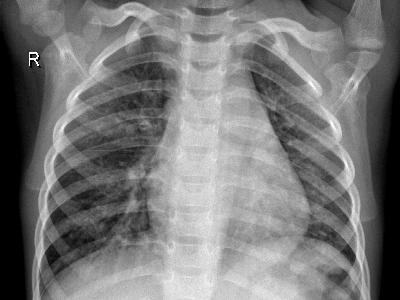
\includegraphics[width=\textwidth]{imgs/Pneumonia-Viral (1).jpg}
         \caption{}
         \label{fig:example_pneumonia_viral}
     \end{subfigure}
     \hfill
     \caption{Example images from the dataset. Patient is healthy (a), with Covid-19 (b), Bacterial Pneumonia (c) and Viral Pneumonia (d).}
     \label{fig:dataset_examples}
\end{figure}

\subsection{Statistical Analysis}

The four classes of the dataset are distributed as follows: Normal 35.51\%, Pneumonia Bacterial 32.59\%, Pneumonia Viral 17.99\% and Covid-19 13.92\%. This distribution is displayed, in absolute count, on the histogram of Fig. \ref{fig:data_distribution}.

\begin{figure}[htp]
    \centering
    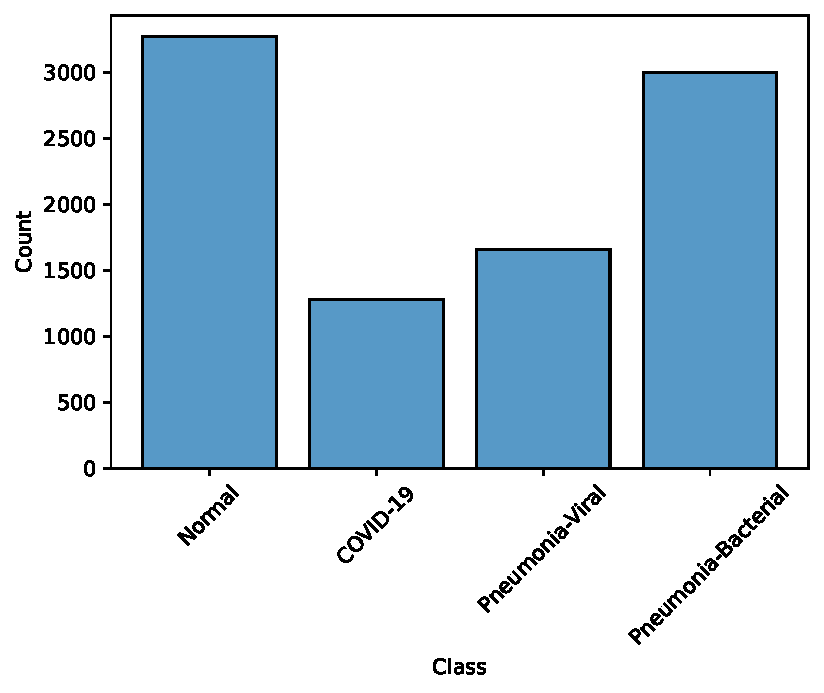
\includegraphics[width=0.4\textwidth]{imgs/data_distribution.pdf}
    \caption{Histogram of the classes distribution within the dataset.}
    \label{fig:data_distribution}
\end{figure}

\section{Applied Machine Learning Methods}
\label{sec:applied_models}

One of the most effective models — i.e., requiring the fewest FLOPS for inference — that achieves State-of-the-Art accuracy on both ImageNet \cite{deng2009imagenet} and typical image classification transfer learning tasks is EfficientNet \cite{tan2019efficientnet}.

EfficientNet offers a family of models (B0 to B7) that represent a good trade-off between efficiency and accuracy on a range of scales by introducing a heuristic method for scaling the model. By using such a scaling heuristic, the efficiency-focused base model (B0) can outperform models at all scales without having to perform a thorough grid-search of the hyperparameters.

The authors used the transfer learning technique on top of the EfficientNet, so only the last layer is updated in size and weights. This means that only a small portion of the model parameters are trainable. Namely, 7.56\% (331,524 out of 4,383,655) and 3.55\% (397,572 out of 11,184,179) for the EfficientNetB0 and EfficientNetB3, respectively.

To infer the benefits of the transfer learning technique, a custom designed \gls{cnn} was also implemented and trained with the same assumptions as the EfficientNet based models.

\subsection{Data Preprocessing}

As described on Table \ref{tab:efficientnet_resolutions}, the different base models of EfficientNet require different input resolutions and so, the multiple resolutions of the images from the dataset must be resized to the corresponding requirement. For the \gls{cnn} model the authors chose the same input size has the EfficientNetB3 network.

The textual classes where mapped to numerical values as part of this step.

These are, actually, the only requirements since the EfficientNet expects full RGB images in the range of [0, 255] given that normalization is included as part of the model.

On the other hand, for the \gls{cnn} model, the input should be a normalized grayscale image.

\begin{table}[htp]
\centering
\caption{Image resolution for each EfficientNet base model.}
\label{tab:efficientnet_resolutions}
\begin{tabular}{ccc}
Base Model     & Resolution     & Channels \\ \hline
EfficientNetB0 & $224 \times 224$ & 3        \\
EfficientNetB1 & $240 \times 240$ & 3        \\
EfficientNetB2 & $260 \times 260$ & 3        \\
EfficientNetB3 & $300 \times 300$ & 3        \\
EfficientNetB4 & $380 \times 380$ & 3        \\
EfficientNetB5 & $456 \times 456$ & 3        \\
EfficientNetB6 & $528 \times 528$ & 3        \\
EfficientNetB7 & $600 \times 600$ & 3       
\end{tabular}
\end{table}

\subsection{Data Augmentation}

To try avoiding over-fitting, the authors opted to apply some random transformations to some of the base images. These transformations are detailed on Table \ref{tab:data_augment}.

\begin{table}[htp]
\centering
\caption{Values used in the transformations for the data augmentation.}
\label{tab:data_augment}
\begin{tabular}{ccc}
             & From & To   \\ \hline
Zoom         & 95\%  & 105\% \\
Brightness   & 90\%  & 100\% \\
Height Shift & -5\%  & 5\%   \\
Width Shift  & -5\%  & 5\%   \\
Rotation     & -10º & 10º 
\end{tabular}
\end{table}

\subsection{CNN Model}

To have a benchmark model, a custom \gls{cnn} model (see Fig. \ref{fig:subnetwork_cnn}) was implemented with all 5,380,996 parameters trainable. 

The goal of this network is to access if a simpler model with more parameters offers any advantages compared to the models based on the EfficientNet, that have less trainable parameters but have a more capable, pre-trained, backbone. 

\begin{figure}[htp]
    \centering
    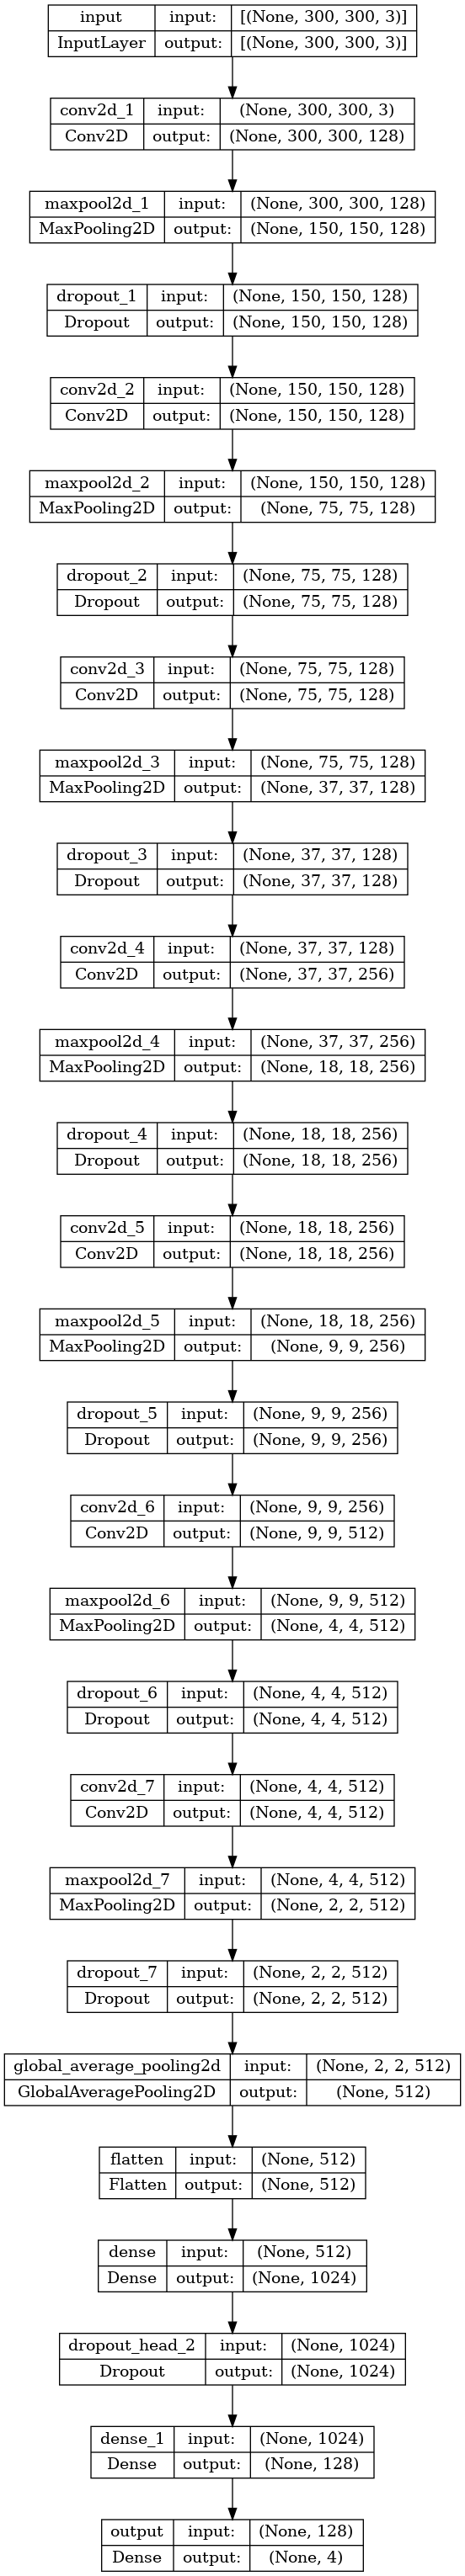
\includegraphics[height=0.95\textheight]{imgs/model_plot_cnn.png}
    \caption{Full \gls{cnn} network implemented.}
    \label{fig:subnetwork_cnn}
\end{figure}

\subsection{EfficientNet Models}

As mentioned previously, the base of the implemented model is the EfficientNet trained with ImageNet dataset. For the problem of this project, the last layer of the base EfficientNet is substituted by a \textit{sub-network} that will be trained with our dataset.

This \textit{sub-network} (see Fig. \ref{fig:subnetwork}) is composed by a Normalization, a Dropout and two Dense layers. The Normalization layer will normalize the values outputed from the pre-trained network to our specific problem, while the Dropout is there to try to prevent over-fitting the data, but only during the training phase.

\begin{figure}[htp]
    \centering
    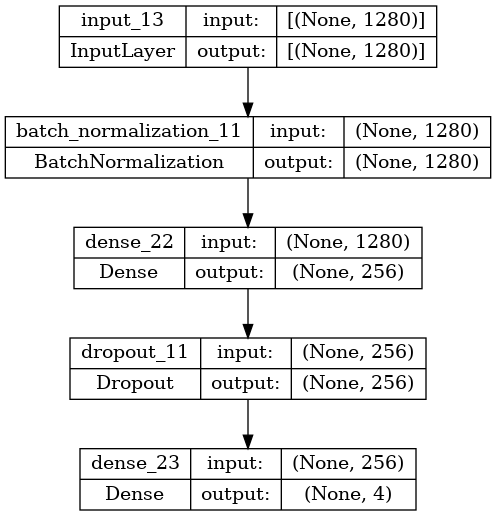
\includegraphics[width=0.4\textwidth]{imgs/model_plot.png}
    \caption{\textit{Sub-network} attached to the second-to-last layer of EfficientNet.}
    \label{fig:subnetwork}
\end{figure}

\subsection{Training}
\label{sec:training}

The training of the models was done in a maximum of 30 epochs. Yet, if in four consecutive epochs, the validation loss did not drop more than 0.01, then the training procedure would reach an early stop.

The authors also decided to reduce the learning rate if the same validation loss did not improve more than $10^{-4}$ during two consecutive epochs. The initial learning rate was set to $10^{-3}$ and, at each time a learning rate reduction was required, the previous value was multiplied by 0.1, down to the minimum learning rate of $10^{-7}$.

The dataset was, also, split into three subsets: train (81\%), validation (10\%) and test (9\%). 

The chosen basis used were the B0 and B3 networks. The EfficientNetB0 was chosen to assess the performance of the most basic (and so, faster to train) model. In counterpart, the EfficientNetB3 was the most complex model of the family that could be trained in a reasonable amount of time.

\section{Results}

The first major disparity between the training of all models is the amount of epochs taken to reach convergence. As explained above, convergence is reached when the model can not improve the loss on the validation set for four consecutive epochs.

Although the random nature of the training may have some impact on the amount of epochs, it should not explain alone the difference of 10 epochs, i.e., while the model based on the EfficientNetB0 took 17 epochs to reach convergence, the model based on the EfficientNetB3 took 27. 

In contrast, the simpler \gls{cnn} model -- although having far more parameters -- reached the early stop criteria at epoch 11. This seams to suggests that the complexity of the model has a greater impact on the training length that the amount of parameters by themselves.

A more detailed comparison between the models follows on the next sections, yet some descriptive metrics of the train models (computed using a macro average) are shown on table \ref{tab:train_results}. As expected, the more complex model improves all the metrics compared to all others, at the cost of training time. But, notice, how the simpler \gls{cnn} model outperforms (in most metrics) the most basic EfficientNet model, despite receiving 67\% less pixels as input. This may be the first indication that the pre-trained weights are introducing some added strain on the training and another early stop criteria should be used.

\begin{table}[htp]
\centering
\caption{Descriptive metrics for the trained models. Values obtained using macro averages.}
\label{tab:train_results}
\begin{tabular}{ccccc}
               & Accuracy & Precision & Recall & F1-score \\ \hline
CNN            & 0.85     & 0.83      & 0.82   & 0.83     \\
EfficientNetB0 & 0.84     & 0.83      & 0.81   & 0.82     \\
EfficientNetB3 & 0.87     & 0.87      & 0.85   & 0.86    
\end{tabular}
\end{table}


\subsection{Loss}

The loss function evaluation for either the training and validation data are shown on Figs. \ref{fig:cnn_loss}, \ref{fig:b0_loss} and \ref{fig:b3_loss} for the \gls{cnn}, EfficientNetB0 and EfficientNetB3 models, respectively.

Both EfficientNet behaviours are very similar, decreasing sharply in the first few epochs and never diverging from one another. 

Interestingly, the \gls{cnn} model started with far lower losses than the EfficientNet counterparts, almost 75\% less, which may be due to pure chance or it is an indication that, in such early stage, the pre-trained weights are introducing a larger error that the \textit{sub-network} is not yet able to compensate.

\begin{figure}[htp]
    \centering
    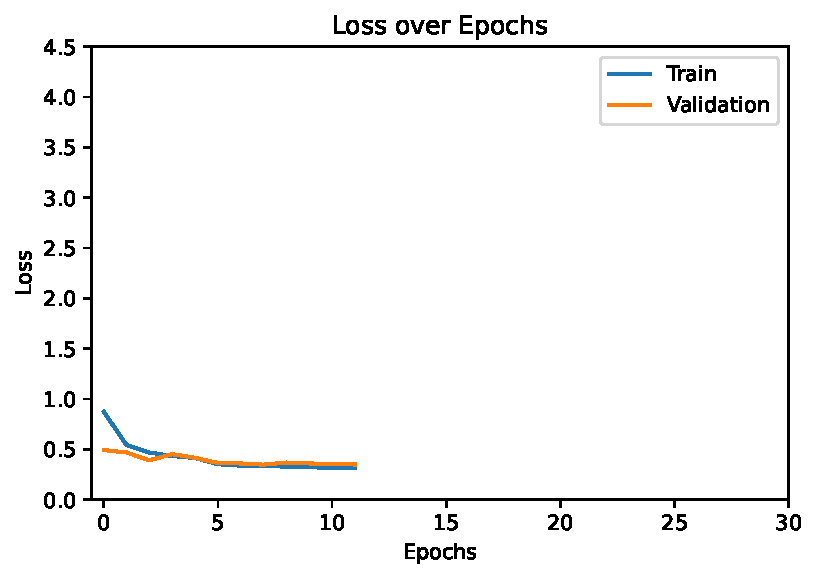
\includegraphics[width=0.4\textwidth]{imgs/cnn_loss.pdf}
    \caption{Loss evolution for the train and validation data, using the \gls{cnn} model.}
    \label{fig:cnn_loss}
\end{figure}

\begin{figure}[htp]
    \centering
    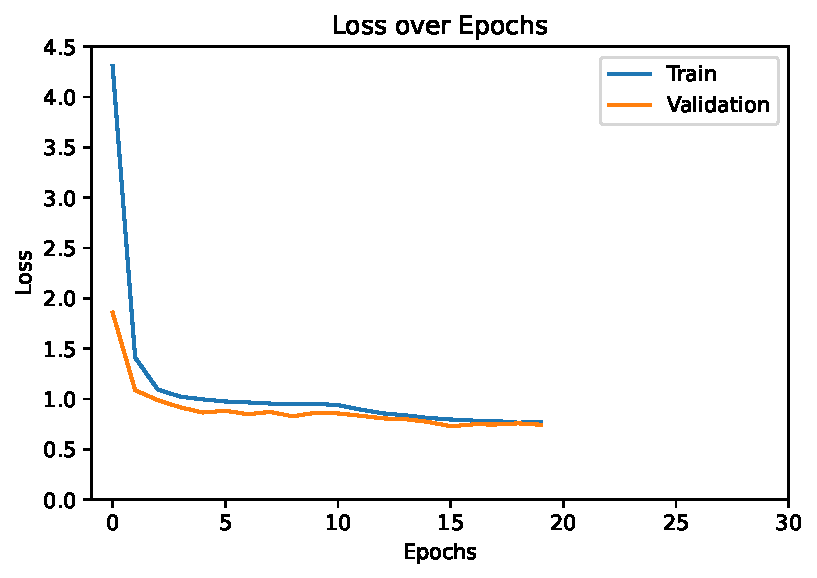
\includegraphics[width=0.4\textwidth]{imgs/EfficientNetB0_loss.pdf}
    \caption{Loss evolution for the train and validation data, using EfficientNetB0 as basis.}
    \label{fig:b0_loss}
\end{figure}

\begin{figure}[htp]
    \centering
    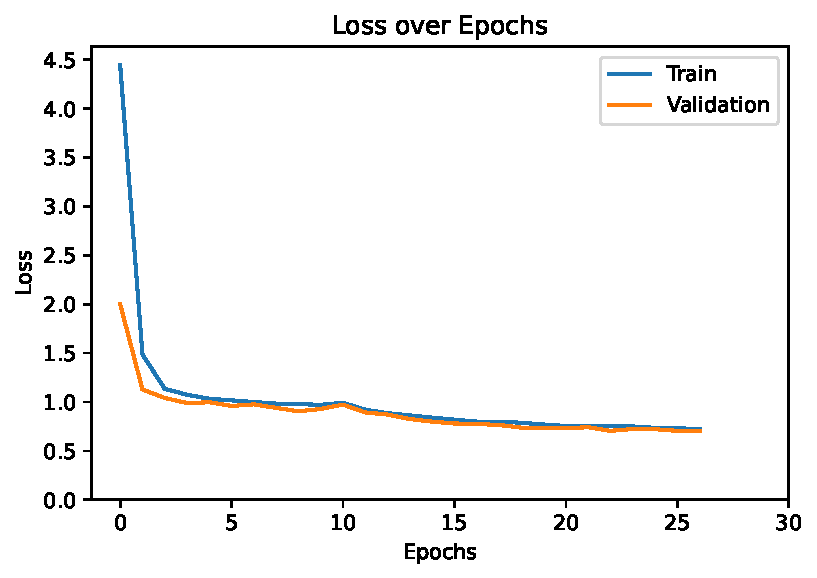
\includegraphics[width=0.4\textwidth]{imgs/EfficientNetB3_loss.pdf}
    \caption{Loss evolution for the train and validation data, using EfficientNetB3 as basis.}
    \label{fig:b3_loss}
\end{figure}

\subsection{Accuracy}

Similarly, the evolutions of the accuracy are shown on Figs. \ref{fig:cnn_accu}, \ref{fig:b0_accu} and \ref{fig:b3_accu}. 

This metric, for the EfficientNet models, tends to be higher on the validating set, which happens because of the Dropout layer (see Fig. \ref{fig:subnetwork}). When training, a portion of the features are set to zero, by this layer, to avoid overfitting, at the cost accuracy while training. When validating, this behaviour does not happen and, logically, more features lead to a higher accuracy.

In contrast, the \gls{cnn} actually switches this trend and ends up with an higher accuracy on the train set than on the validation set. This can be explained twofold: i) in the \gls{cnn} model there are two Dense layers after the last Dropout layer, while in the EfficientNet models the Dropout layer is directly connected to the output and ii) the random nature of the data split may just selected a "worst case scenario" for this metric. Solutions and further details will be discussed in the coming sections.

\begin{figure}[htp]
    \centering
    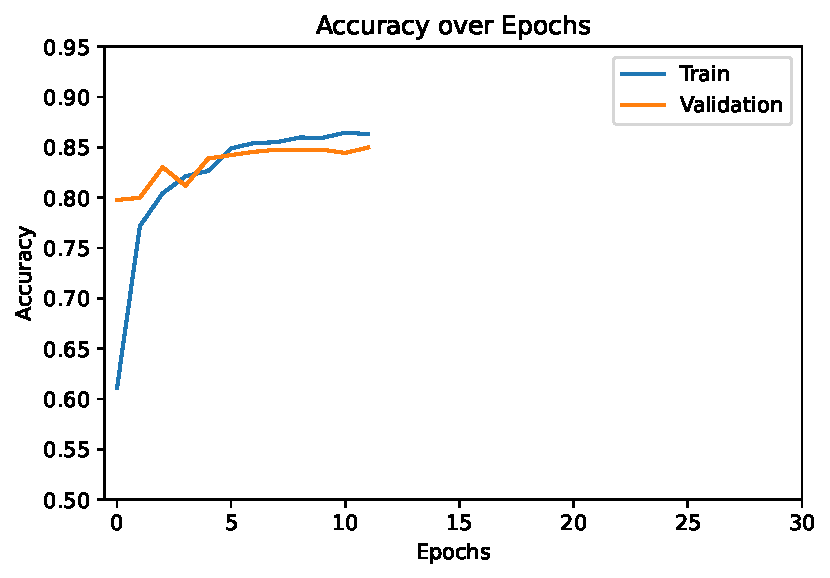
\includegraphics[width=0.4\textwidth]{imgs/cnn_accu.pdf}
    \caption{Accuracy evolution for the train and validation data, using the \gls{cnn} model.}
    \label{fig:cnn_accu}
\end{figure}

\begin{figure}[htp]
    \centering
    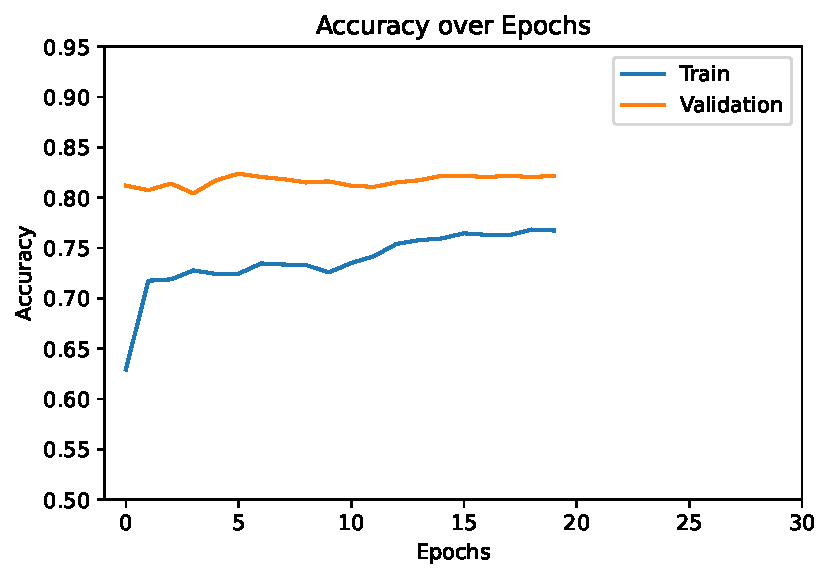
\includegraphics[width=0.4\textwidth]{imgs/EfficientNetB0_accu.pdf}
    \caption{Accuracy evolution for the train and validation data, using EfficientNetB0 as basis.}
    \label{fig:b0_accu}
\end{figure}

\begin{figure}[htp]
    \centering
    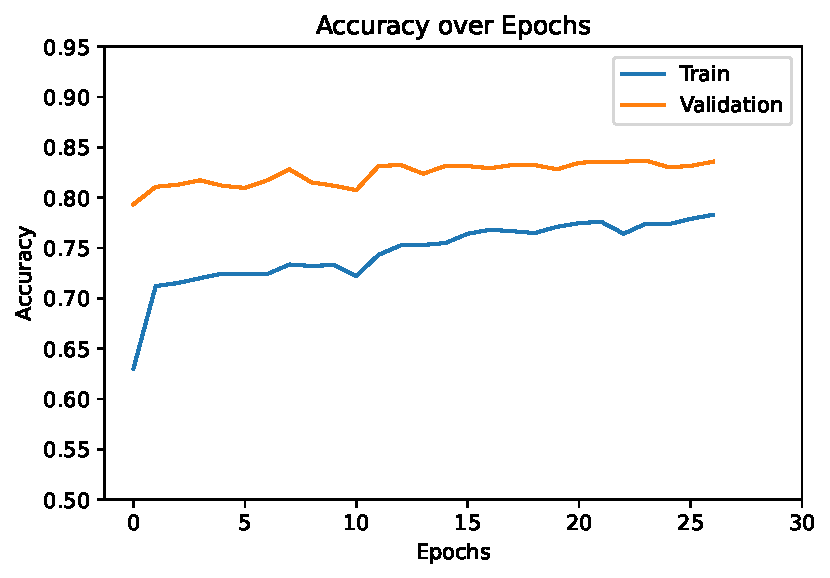
\includegraphics[width=0.4\textwidth]{imgs/EfficientNetB3_accu.pdf}
    \caption{Accuracy evolution for the train and validation data, using EfficientNetB3 as basis.}
    \label{fig:b3_accu}
\end{figure}



\subsection{Learning Rate}

As expected, the learning rate behaviours are very similar (see Figs. \ref{fig:cnn_lr}, \ref{fig:b0_lr} and \ref{fig:b3_lr}). 

This hyperparameter has a staircase like behaviour that is caused by a stagnation in the validation loss, as explained on section \ref{sec:training}. 

Logically, to have four consecutive epochs with stagnation, first there must be two, and that is why all three models have similar curves at the end.

\begin{figure}[htp]
    \centering
    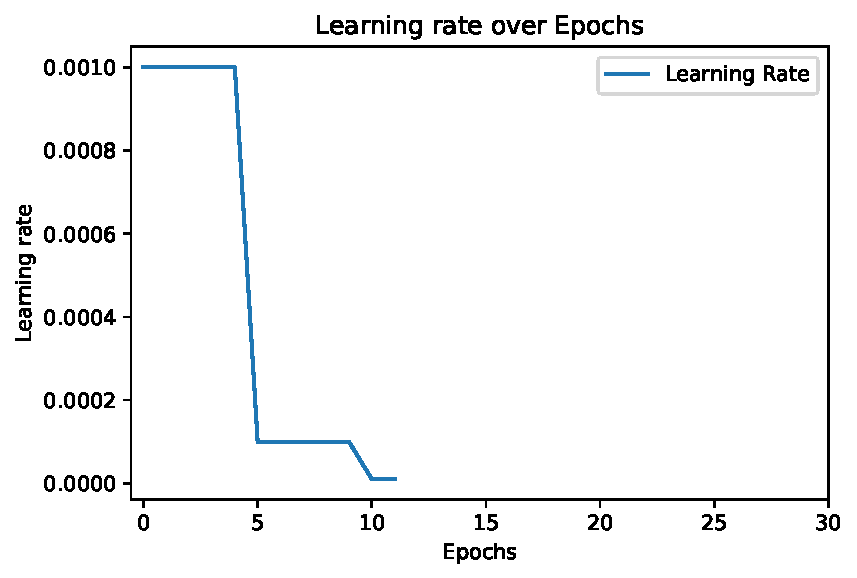
\includegraphics[width=0.4\textwidth]{imgs/cnn_lr.pdf}
    \caption{Learning rate evolution for the train and validation data, using the \gls{cnn} model.}
    \label{fig:cnn_lr}
\end{figure}

\begin{figure}[htp]
    \centering
    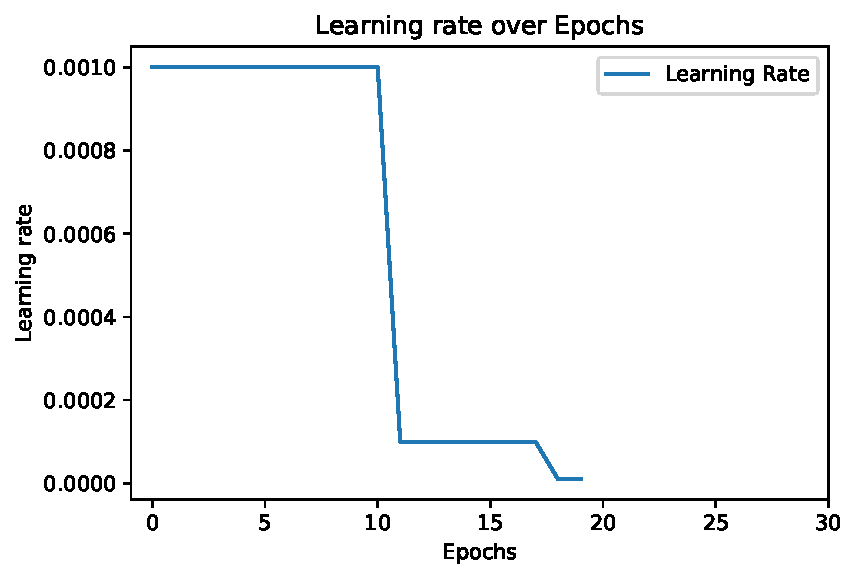
\includegraphics[width=0.4\textwidth]{imgs/EfficientNetB0_lr.pdf}
    \caption{Learning rate evolution for the train and validation data, using EfficientNetB0 as basis.}
    \label{fig:b0_lr}
\end{figure}

\begin{figure}[htp]
    \centering
    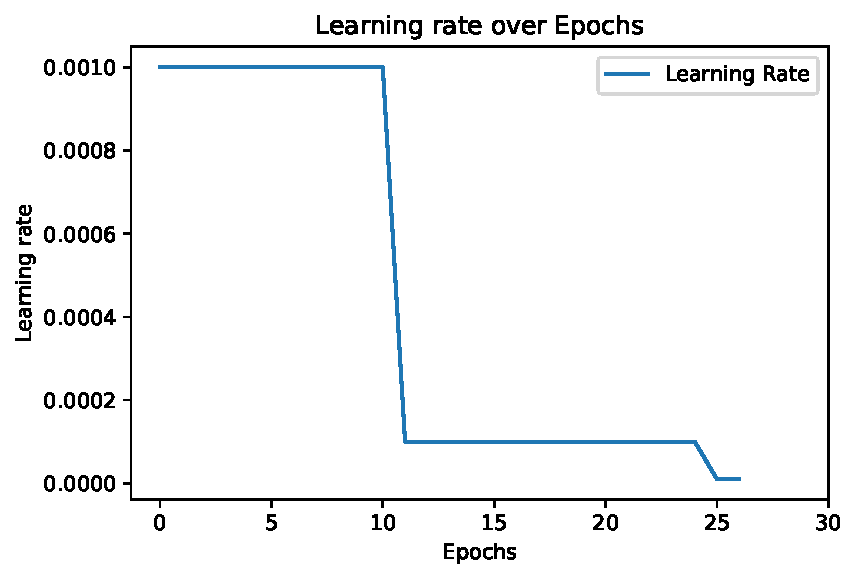
\includegraphics[width=0.4\textwidth]{imgs/EfficientNetB3_lr.pdf}
    \caption{Learning rate evolution for the train and validation data, using EfficientNetB3 as basis.}
    \label{fig:b3_lr}
\end{figure}

\subsection{Confusion}

Finally, the confusion matrices are presented on Figs. \ref{fig:cnn_confusion}, \ref{fig:b0_confusion} and \ref{fig:b3_confusion}.

These confusion matrices are backed by Table \ref{tab:f1_comparison}. Combined, they state that even though the COVID-19 class was the one with less data, it is the one with the highest F1-score for all models. This metric is lower in both pneumonia classes, which was expected given that, even if the cause is distinct, the disease is the same and the symptoms should be similar, creating a greater difficulty to differentiate them.
 
It is noticeable that the \gls{cnn} model implemented reaches higher F1-Scores than the EfficientNetB0 for the Normal and Viral Pneumonia classes, which may be explained by the higher resolution images fed to the prior model.

\begin{figure}[htp]
    \centering
    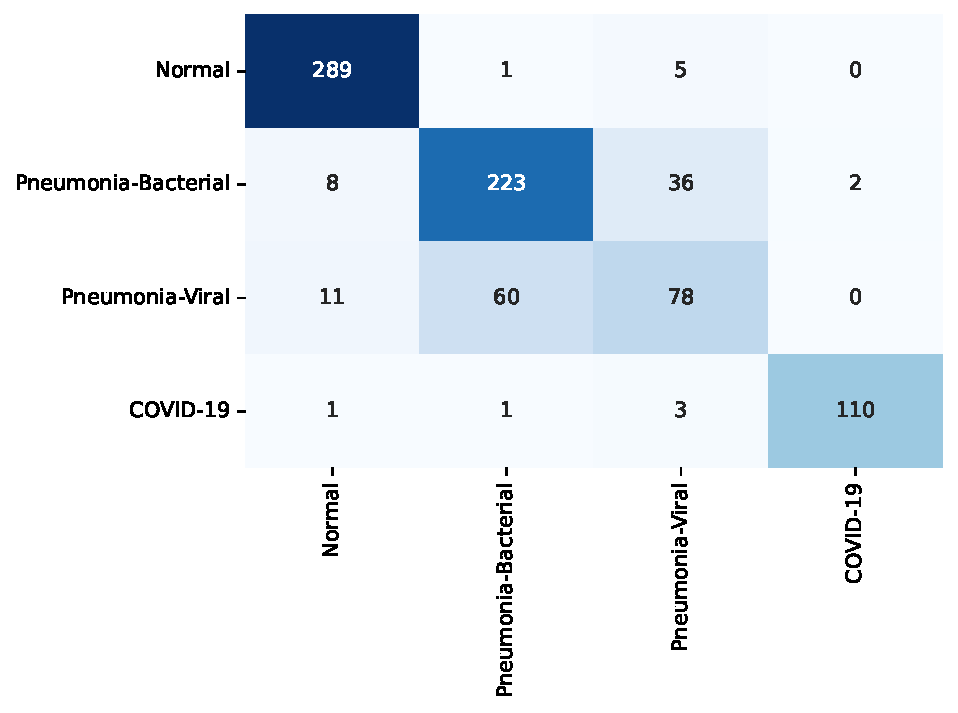
\includegraphics[width=0.4\textwidth]{imgs/cnn_confusion.pdf}
    \caption{Confusion matrix for the test data, using the \gls{cnn} model.}
    \label{fig:cnn_confusion}
\end{figure}

\begin{figure}[htp]
    \centering
    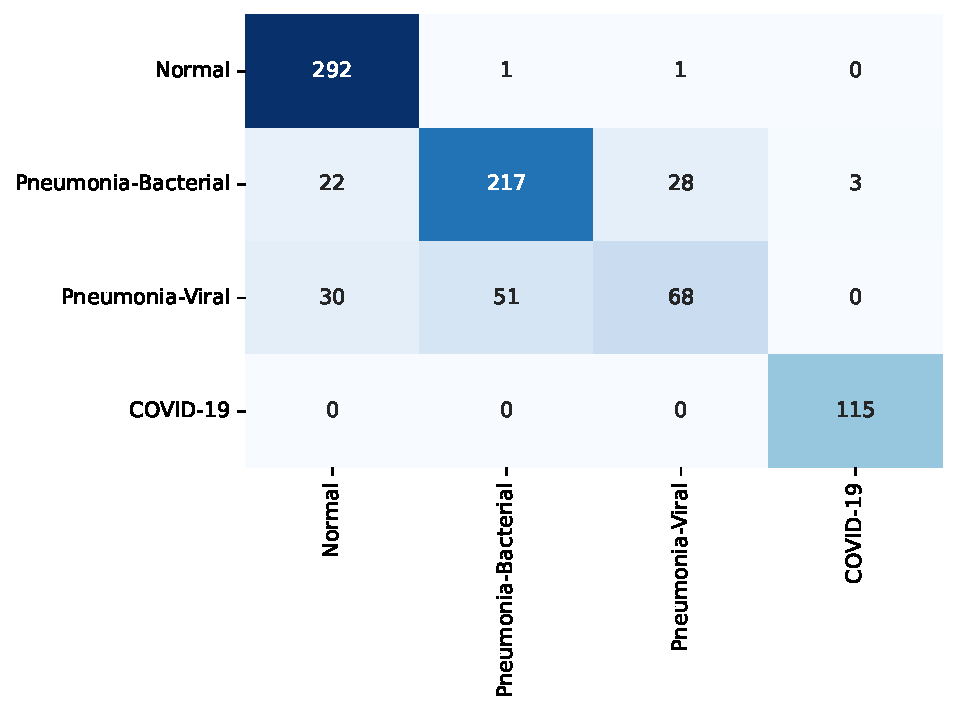
\includegraphics[width=0.4\textwidth]{imgs/EfficientNetB0_confusion.pdf}
    \caption{Confusion matrix for the test data, using EfficientNetB0 as basis.}
    \label{fig:b0_confusion}
\end{figure}

\begin{figure}[htp]
    \centering
    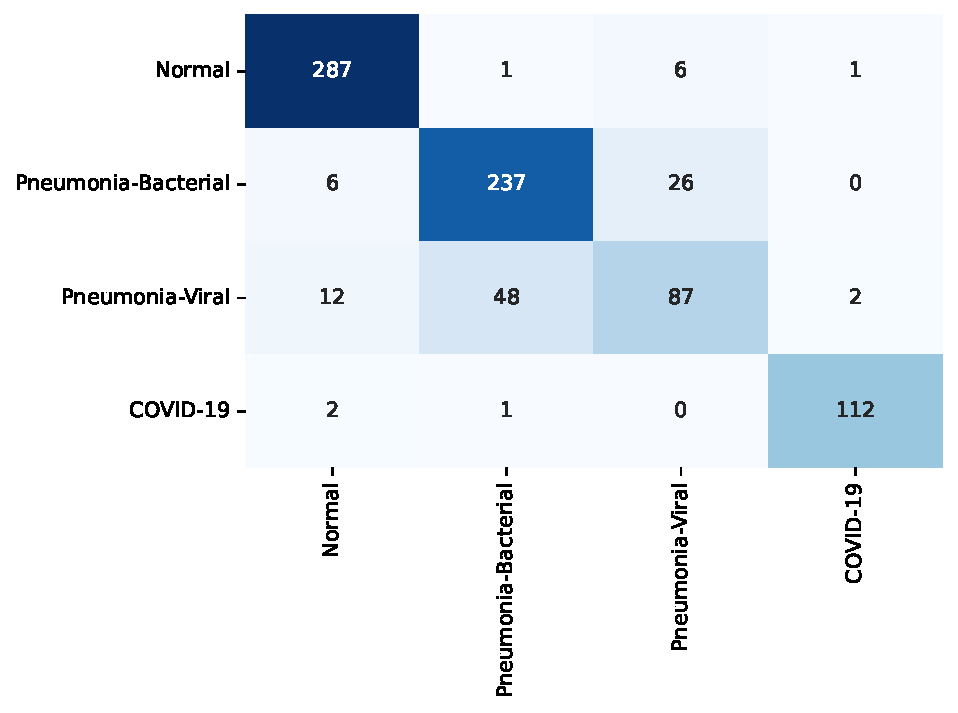
\includegraphics[width=0.4\textwidth]{imgs/EfficientNetB3_confusion.pdf}
    \caption{Confusion matrix for the test data, using EfficientNetB3 as basis.}
    \label{fig:b3_confusion}
\end{figure}

\begin{table}[htp]
\centering
\caption{F1-score comparison of the trained models, for all the classes.}
\label{tab:f1_comparison}
\begin{tabular}{cccc}
                    & CNN & EfficientNetB0 & EfficientNetB3 \\ \hline
Normal              & 0.96 & 0.92           & 0.95           \\
Bacterial Pneumonia  & 0.81 & 0.81           & 0.85           \\
Viral Pneumonia      & 0.58 & 0.55           & 0.65           \\
COVID-19            & 0.97 & 0.99           & 0.97          
\end{tabular}
\end{table}

\section{Conclusion}

The advantages of \gls{ml}, \glspl{cnn} and the transfer learning technique have become clear. 

In this work the authors proved the benefits of using such technologies for an early diagnosis of pneumonia and COVID-19. Although the accuracy reached is not high enough for use in the real world scenarios, room for improvement still exists. 

While doctors should never by replaced by \gls{ml} models, their great contribute to society can be greatly enhanced by working together with this powerful new tools.

Regarding the selected and implemented models, some interesting conclusions can be attained. Contrarily to initially expected by the authors, the transfer learning used in the EfficientNetB0 model provided little or insignificant improvements. This may be because the EfficientNet family is more suited to classification tasks with more categories. The image resolution is also a variable along the models and, certainly, impacts all metrics analysed. Nontheless, the EfficientNetB3 model with transfer learning corresponded to the expectations and delivered the best overall performance.

Moving from the EfficientNetB0 to the EfficientNetB3 provided some improvements, but it remains unclear if the more complex models (like the B5 or even the B7) would provide a bigger jump from the simpler \gls{cnn} model or not.

Lastly, it has been realized that it is not only the complexity or the number of trainable parameters alone that affect the training time but a balance between these hyper parameters.


\subsection{Future Work}

One not explored path in this work was to train the full EfficientNet networks, i.e., the last \textit{sub-network} as well as the backbone network, substituting the pre-trained weights. Given the amount of parameters combined with the size of the dataset this taske would be extremely time intensive, but would clarify the impact of the pre-trained weights on the results achieved.

Additionally, a fixed \gls{cnn} model should be implemented, with the last Dropout layer directly connected to the output layer, so a direct comparison could be made.

Finally, in insight, the early stop strategy adopted may have led to some inaccuracies in all models. A longer training, with a more difficult to reach stopping criterion, should be adopted to infer the possible benefits that come with it.

\FloatBarrier
\printbibliography

\end{document}
